\documentclass{article}
\usepackage{graphicx, amsmath, float, siunitx, hyperref, mathtools} % Required for inserting images
\usepackage[ngerman]{babel}
\usepackage{biblatex, csquotes}
\addbibresource{refs.bib}
\usepackage[
  locale=DE,
  separate-uncertainty=true,
  per-mode=symbol
]{siunitx}

\DeclareSIUnit\gauss{G}

\newcommand{\abb}{{\color{red}\textbf{{ABB.XYZ}}} }
\newcommand{\Oszi}{Oszilloskop }

\usepackage{caption}
\usepackage{subcaption}

\usepackage{csvsimple}
\usepackage{comment}
\usepackage{booktabs}

\title{Praktikum V - Kern- und Teilchenphysik\\Versuch 521 - $\gamma$-Spektroskopie mit Szintillations- und Halbleiterdetektoren}

\author{Tom Chelius und Alican Özcagi}
\date{24. April 2025}

\begin{document}

\maketitle
\tableofcontents

\newpage
\section{Einleitung}

\section{Theorie}

\section{Voraufgabe}
Es sollte für ein gegebenes Spektrum ein Skript geschrieben werden, womit es möglich ist die Spektrallinien zu analysieren. Hierbei wurde eine Anpassungsfunktion der Form
\begin{equation}
    H + A \cdot \exp{\frac{-(x_i-\mu_i )^2}{2 \sigma_i^2}}
\end{equation}
verwendet und an die jeweiligen gaußförmigen Linien angepasst, die Anpassungsparameter sind in Tabelle \ref{tab:voraufgabe} zu sehen und die Anpassungen an den Graphen in \ref{}


\begin{table}
    \centering
    \begin{tabular}{|c|c|c|c|c|c|c|} \hline
      Peaknummer & A & $\Delta A$ & $\mu$ & $\Delta \mu$ & $\sigma$ & $\Delta \sigma$\\ \hline \hline
      1 & 457 & 20 & 330,18 & 0,118 & 35,11 & 0,2295 \\ \hline
      2 & 48 & 106 & 599,44 & 76,846 & 67,21 & 396,4932 \\ \hline
      3 & 66 & 97 & 796,09 & 1408,613 & 93,56 & 867,4174 \\ \hline
      4 & 250 & 891 & 922,1 & 3,805 & 50,11 & 6,9929 \\ \hline
      5 & 11352 & 121842 & 3280,98 & 9,108 & 154,67 & 15,4185 \\ \hline
      6 & 32797 & 72979 & 3920,76 & 1,437 & 155,2 & 1,4584 \\ \hline
    \end{tabular}
    \caption{Anpassung an spectrum.txt aus der Voraufgabe}
    \label{tab:voraufgabe}
\end{table}

\begin{figure}
    \centering
    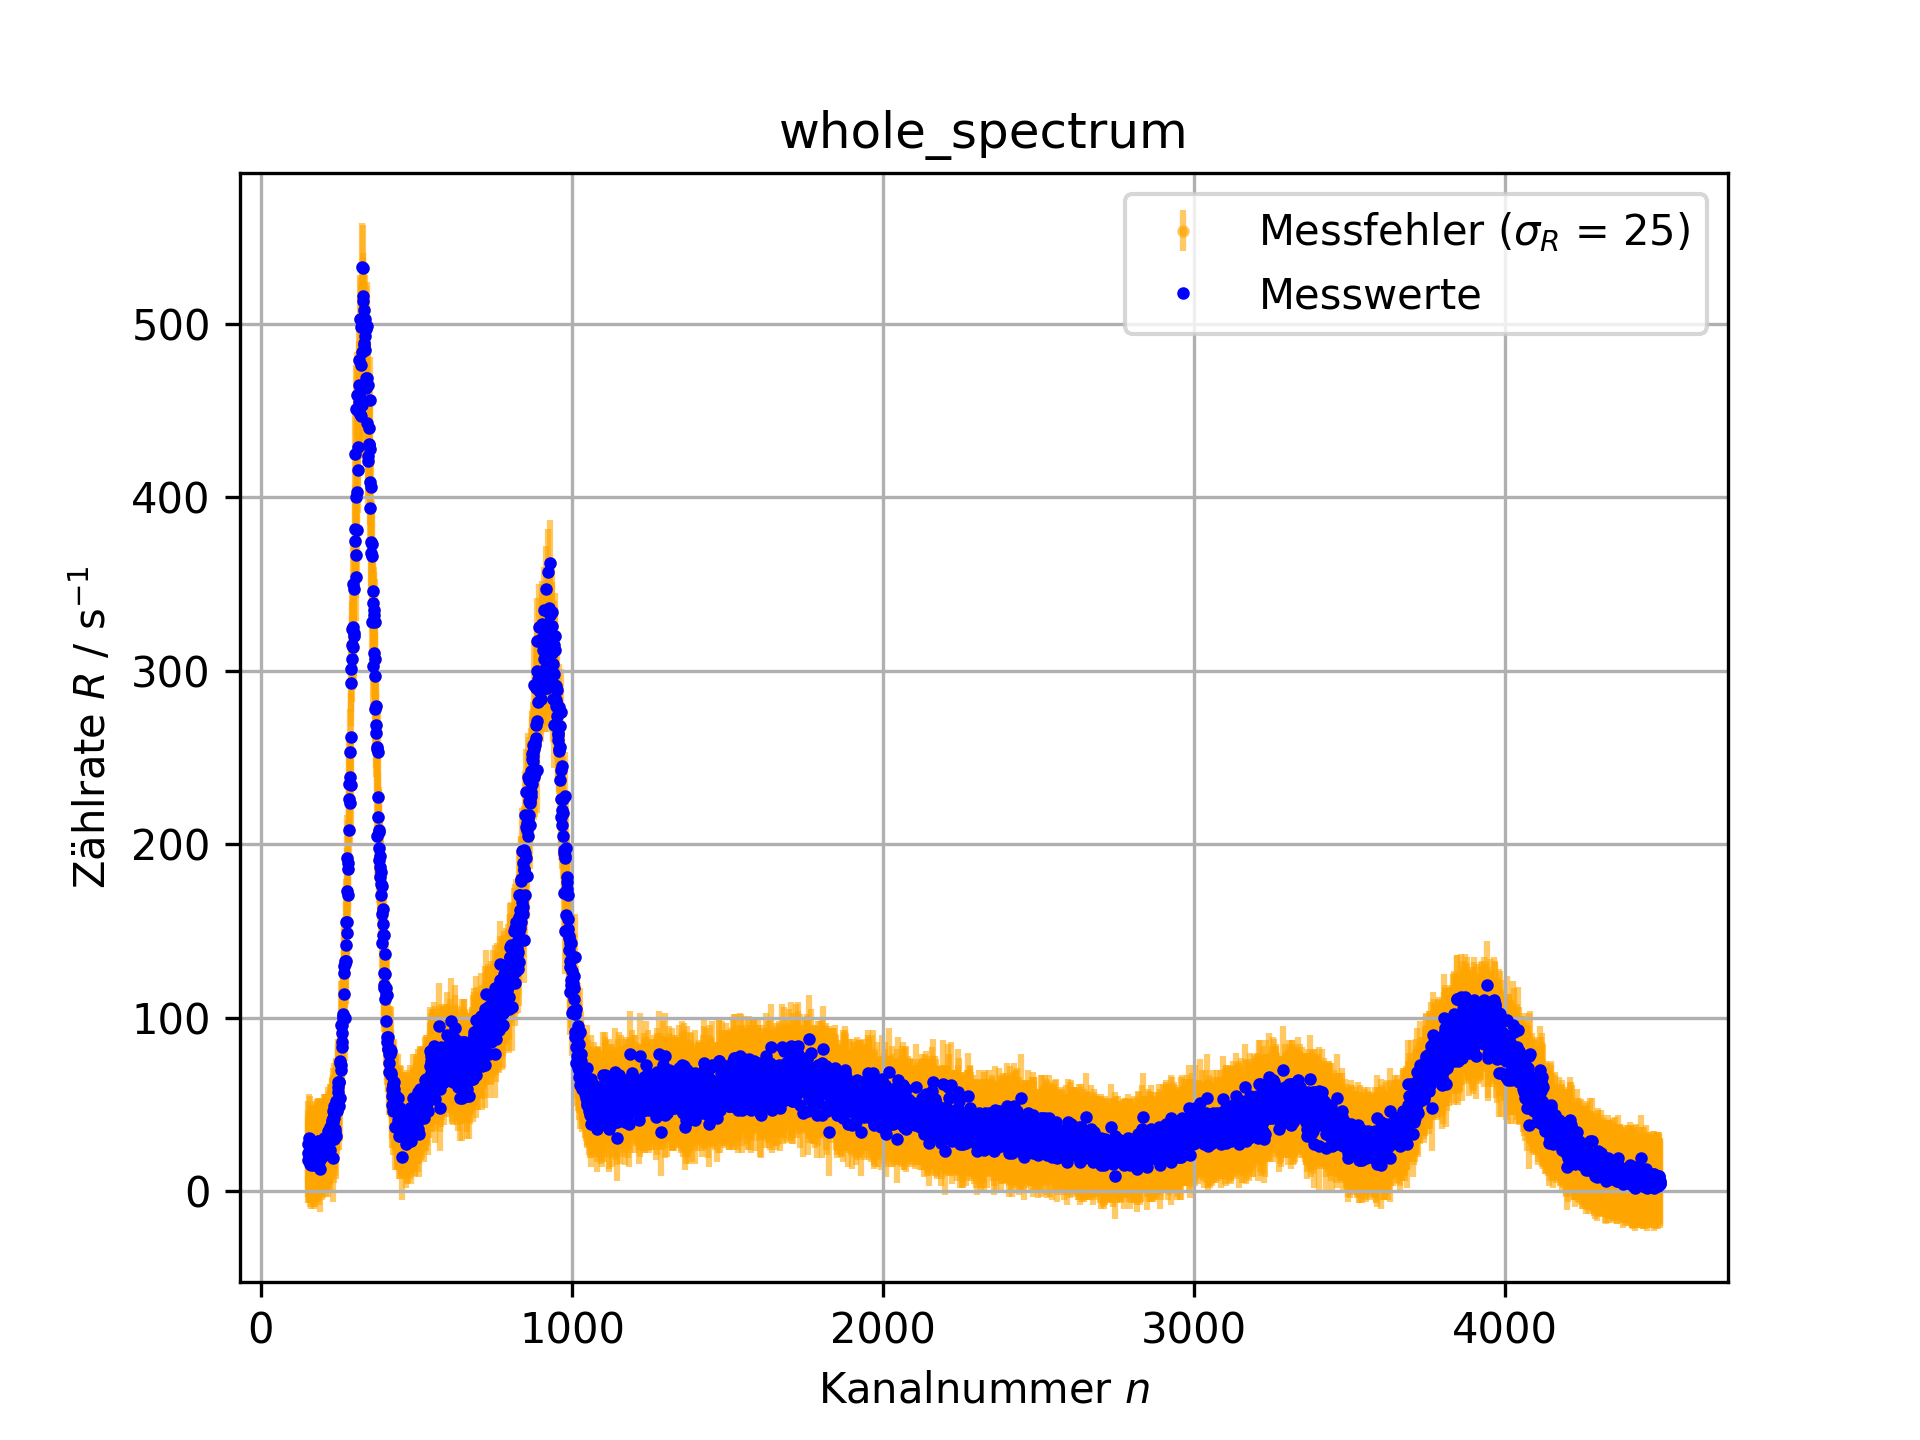
\includegraphics[width=1\linewidth]{/figures/whole_spectrum.png}
    \caption{Anpassungsfunktion}
    \label{fig:voraufgabeFig}
\end{figure}

\section{NaI-Szintillationsdetektor}

\begin{table}
  \centering
  \begin{tabular}{|c|c|c|c|c|c|c|} \hline
    Peaknummer & A & $\Delta A$ & $\mu$ & $\Delta \mu$ & $\sigma$ & $\Delta \sigma$\\ \hline \hline
    1 & 11716 & 7199692 & 846,5 & 77,379 & 248,07 & 368,5535 \\ \hline
    2 & 23655 & 52474412 & 1289,08 & 12668,174 & 574,0 & 6040,7053 \\ \hline
    3 & 172257 & 206990 & 5600,18 & 0,191 & 164,78 & 0,1426 \\ \hline
    4 & 60052 & 189125 & 9710,81 & 1,454 & 211,13 & 1,8219 \\ \hline
    5 & 60918 & 445230 & 11010,8 & 1,556 & 248,78 & 4,2583 \\ \hline
    6 & 14320 & 194791 & 116,23 & 0,039 & 12,77 & 0,0817 \\ \hline
    7 & 101370 & 340523 & 407,14 & 0,029 & 37,51 & 0,0362 \\ \hline
    8 & 47169 & 15716111 & 844,49 & 14,11 & 153,74 & 51,765 \\ \hline
    9 & 66879 & 347400 & 1129,13 & 0,11 & 50,28 & 0,1257 \\ \hline
    10 & 15672 & 2607443 & 2157,14 & 12,463 & 90,53 & 23,8622 \\ \hline
    11 & 40336 & 762119 & 2998,86 & 1,492 & 111,62 & 2,7803 \\ \hline
    12 & 6670 & 143922 & 6570,57 & 26,448 & 165,45 & 48,2298 \\ \hline
    13 & 6023 & 64572 & 8062,55 & 19,467 & 184,6 & 35,901 \\ \hline
    14 & 12093 & 242589 & 9175,25 & 13,749 & 245,97 & 46,1394 \\ \hline
    15 & 5894 & 77840 & 11617,48 & 31,117 & 227,29 & 60,6962 \\ \hline
  \end{tabular}
  \caption{Anpassung an spectrum.txt aus der Voraufgabe}
  \label{tab:voraufgabe}
\end{table}

\section{HPGe-Halbleiterdetektore}

\begin{table}
  \centering
  \begin{tabular}{|c|c|c|c|c|c|c|} \hline
    Peaknummer & A & $\Delta A$ & $\mu$ & $\Delta \mu$ & $\sigma$ & $\Delta \sigma$\\ \hline \hline
    1 & 268 & 475 & 15154,28 & 0,431 & 8,85 & 0,4008 \\ \hline
    2 & 80535 & 85935 & 6863,19 & 0,001 & 6,74 & 0,0004 \\ \hline
    3 & 7470 & 8188 & 12170,32 & 0,01 & 8,09 & 0,0065 \\ \hline
    4 & 6640 & 7576 & 13822,81 & 0,012 & 8,27 & 0,0081 \\ \hline
    5 & 55334 & 85353 & 1262,08 & 0,001 & 4,9 & 0,0006 \\ \hline
    6 & 12267 & 27685 & 2537,12 & 0,004 & 5,34 & 0,0044 \\ \hline
    7 & 31697 & 46588 & 3570,23 & 0,001 & 5,73 & 0,0013 \\ \hline
    8 & 983 & 3345 & 3814,6 & 0,096 & 5,89 & 0,1043 \\ \hline
    9 & 2246 & 4814 & 4263,47 & 0,03 & 5,98 & 0,0297 \\ \hline
    10 & 2828 & 5437 & 4604,36 & 0,023 & 6,12 & 0,0223 \\ \hline
    11 & 6900 & 9587 & 8079,55 & 0,01 & 6,96 & 0,0082 \\ \hline
    12 & 2003 & 4136 & 8996,95 & 0,049 & 7,35 & 0,0482 \\ \hline
    13 & 6336 & 8281 & 10000,47 & 0,012 & 7,64 & 0,0095 \\ \hline
    14 & 3990 & 5410 & 11264,0 & 0,02 & 7,83 & 0,0164 \\ \hline
    15 & 577 & 2166 & 11304,05 & 0,206 & 7,41 & 0,2777 \\ \hline
    16 & 5018 & 6576 & 11535,89 & 0,017 & 7,89 & 0,0131 \\ \hline
    17 & 6364 & 6777 & 14605,91 & 0,013 & 8,65 & 0,0084 \\ \hline

  \end{tabular}
  \caption{Anpassung an spectrum.txt aus der Voraufgabe}
  \label{tab:voraufgabe}
\end{table}

\newpage
\printbibliography[heading=bibintoc]

\end{document}